\documentclass{article}
\usepackage{graphicx}
\usepackage[utf8]{inputenc}
\usepackage{url}
\usepackage{xcolor}


\title{\textsf{nn-dependability-kit} manual \\ \begin{large}(Public version)\end{large}}

\date{February 13th, 2019}

\usepackage{natbib}
\usepackage{graphicx}

\begin{document}

\maketitle

\section{Introduction}

\textsf{nn-dependability-kit} is a research tool with the goal of assisting engineering neural networks for safety-critical domains. 


\section{Availability and License}

The online version of the tool is publicly released under the GNU Affero General Public License (AGPL) Version 3, which is a strong copyleft open source license. 

\vspace{5mm}

\url{https://github.com/dependable-ai/nn-dependability-kit/}



\section{Dependencies and Installation}

Here we list dependencies of $\textsf{nn-dependability-kit}$:
\begin{description}
\item[(Basics)] \texttt{PyTorch} + \texttt{Numpy} + \texttt{matplotlib} + \texttt{jupyter}. 
\item[(Test case generation)] Google optimization research tools, available at \\ {\small\url{https://developers.google.com/optimization/introduction/installing/binary}}

\item[(Verification / static analysis)] \texttt{PuLP} (python-based MILP connector to Coin-or branch and cut (CBC) solver and other solvers)
\begin{itemize}
    \item For Ubuntu users, the CBC solver shipped with PuLP may crash in solving some problems. Therefore, please additionally install GNU GLPK. The static analysis engine assumes that the GLPK solver is installed in the default directory "\texttt{/usr/local/bin/glpsol}". Whenever CBC solver crashes, GLPK solver is automatically triggered as a replacement.
    \item For academic users, we strongly advise to use IBM CPLEX as the underlying solver, as academic partners can retrieve IBM CPLEX for free. For open source solvers, we have experienced multiple times unexpected crashes. Even the above workaround cannot guarantee a crash-free behavior. 
\end{itemize}
\item[(Run-time verification)] \texttt{dd} (binary decision diagram implemented using python)
\end{description}

\textsf{nn-dependability-kit} mainly supports PyTorch. For TensorFlow, the support is currently restricted to formal verification. However, as the input for computing the metrics and the input for building monitors uses numpy arrays rather than native pytorch tensors, it is very easy to use these metrics or to build runtime monitors also with TensorFlow. 


\section{Examples}

Within the source code of \textsf{nn-dependability-kit}, examples are presented as jupyter notebooks to allow step-by-step execution with explanations written as markdown languages.  

\section{How to use \textsf{nn-dependability-kit}}

In the following subsections, we explain the capability of \textsf{nn-dependability-kit}, by traversing the package structure while summarizing key functionality within each package. 

\subsection{Package \texttt{basic}} 

Package \texttt{basic} contains intermediate representation of neural networks (\texttt{neuralnet.py}), as well as converters from Pytorch or Tensorflow models to the intermediate representation used by \textsf{nn-dependability-kit}. The intermediate representation is currently only \emph{used for formal verification purposes}, and it supports only multi-layer perception (MLP) with the following types of layer descriptions. 

\begin{itemize}
    \item Rectified Linear Unit (ReLU)
    \item Exponential linear unit (ELU)
    \item Linear 
    \item Batch normalization layer (BN)
\end{itemize}

Note that \textsf{nn-dependability-kit} also \emph{accepts networks with convolution layers}, when one wants to perform testing, metric, or runtime monitoring. The intermediate representation is \emph{only used for verification purposes} - the background is that we advise to do \emph{assume-guarantee style} formal safety verification by taking only close-to-output layers in a network, and the above types are sufficient to capture close-to-output layers.

To this end, the remaining problem is how to read the user-specified part of the network. The below code snippet demonstrates the use of a helper function \texttt{loadMlpFromTensorFlow} to read the last three layers of a tensorflow model. For tensorflow models, one can use tools such as tensorboard to read the name of each layer as well as the layer type. One prepares two python lists (in the below snippet, \texttt{layersNames} and \texttt{layerTypes}) to store the layer name as well as the corresponding layer type. One should also store the input dimension of the ``truncated network" used for formal verification (in the below snippet, \texttt{inputShape}). Then function \texttt{loadMlpFromTensorFlow} instantiates a model for verification by fetching the corresponding parameters in the tensorflow model. 

\begin{small}
\color{blue}
\begin{verbatim}

from nndependability.basic import tensorflowreader

inputShape = (600, 480, 3)
tfModelPath = "frozen_graph.pb"
layersNames = ["model/FC10/fully_connected", 
               "model/FC11/BatchNorm", 
               "model/Output/fully_connected"]
layerTypes = ["elu", "BN-gamma1", "linear"]
# BN-gamma1 is a special case where BN has parameter gamma being 1
model = tensorflowreader.loadMlpFromTensorFlow(tfModelPath, 
                              layersNames, layerTypes, inputShape)
\end{verbatim}
\end{small}



\subsection{Package \texttt{metrics}}

Package \texttt{metrics} includes functions to compute dependability metrics for neural networks. 


\subsubsection{Perturbation loss metric}

\emph{Perturbation loss metric} contains a set of predefined perturbation directions (representing different effects) and predefined quantity (representing different intensity; can be changed if needed). The goal of this metric is to understand if the neural network under analysis is still able to perform correctly with (slightly) perturbed input. An example of using such a metric can be found in the jupyter notebook \texttt{GTSRB\_AdditionalMetrics.ipynb}.   

The below code snippet explains the workflow. Once when one initiates a metric object, to compute the perturbation loss metric, simply add  input images and corresponding labels (both as numpy arrays) to the metric object. There are multiple options for visualizing the metric, such as computing the maximum or average drop of output probability.  

\begin{small}
\color{blue}
\begin{verbatim}


from nndependability.metrics import PerturbationLoss
metric = PerturbationLoss.Perturbation_Loss_Metric()

...

# Let image be the input of the network, represented as numpy arrays
# Let label be the ground truth of the network, 
# also represented as numpy arrays

metric.addInputs(net, image, label)

...
# Print the maximum quantity of probability drop
metric.printMetricQuantity("MAX_LOSS")

# Print the average quantity of probability drop
metric.printMetricQuantity("AVERAGE_LOSS")

\end{verbatim}
\end{small}


\begin{figure}[ht]
\centering
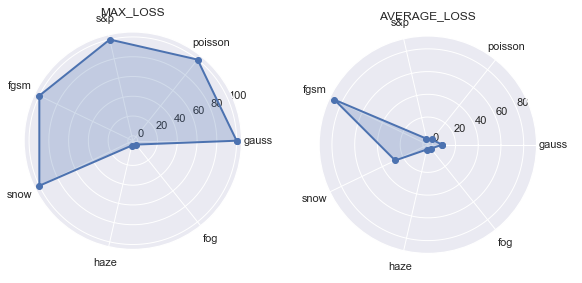
\includegraphics[width=12cm]{fig/PerturbationLoss.png}
\caption{Perturbation loss metric for a traffic sign classification network.}
\label{fig.perturbation}
\end{figure}

Figure~\ref{fig.perturbation} shows the resulting diagram for perturbing a neural network with~7 directions. The \texttt{MAX\_LOSS} diagram indicates that there exists an image in the data set such that perturbing the image by adding the Gaussian noise (\texttt{gauss} in Figure~\ref{fig.perturbation}) leads to~$100\%$ confidence drop, i.e., the network considers the original image to be of class $A$ with $100\%$ probability but the perturbed image is considered to be of class $A$ with $0\%$ probability. 


\subsubsection{Neuron activation pattern metric}

\emph{Neuron activation pattern metric} examines, for input data that is classified into the same class, whether their activation pattern is similar. Due to combinatorial explosion, the similarity of activation patterns is further aggregated into histograms capturing the number of neurons being activated, based on analyzing a user-specified close-to-output neuron layer. An example of using such a metric can be found in the jupyter notebook \texttt{GTSRB\_AdditionalMetrics.ipynb}.

Similar to the code snippet below, one first needs to initiate the metric class, and specify the number of neurons to be monitored (\texttt{sizeOfNeuronsToMonitor}). Subsequently, feed the metric class with 2D numpy arrays where the 1st dimension matches \texttt{sizeOfNeuronsToMonitor} and the 2nd dimension captures the batch size.  

\begin{small}
\color{blue}
\begin{verbatim}

from nndependability.metrics import NeuronActivationPattern

metric = NeuronActivationPattern.Neuron_Activation_Pattern_Metric
                                (num_classes, sizeOfNeuronsToMonitor)

...

# Let "intermediateValues" be the computed pytorch tensor for a 
# particular layer, "predicted" be the originally predicted result,
# and "labels" be the ground truth

metric.addAllNeuronPatternsToClass(intermediateValues.numpy(),
                                    predicted.numpy(), labels.numpy())

...
# Let "class" be an integer value indicating the class index.
metric.printMetricQuantity(class)

\end{verbatim}
\end{small}

Figure~\ref{fig.histogram} shows one histogram for all images being classified by the neural network to class indexed~$0$. 

\begin{figure}[ht]
\centering
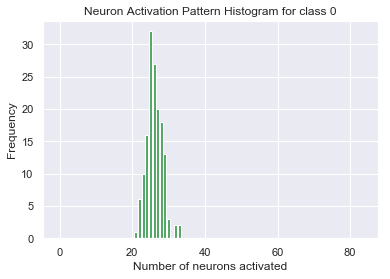
\includegraphics[width=8cm]{fig/ActivationPattern.png}
\caption{Neuron activation pattern represented as a histogram.}
\label{fig.histogram}
\end{figure}

\subsubsection{Scenario k-projection metric}~\label{sub.sec.scenario.k.projection}

\emph{Scenario k-projection coverage} considers how the input data (for training or for testing purposes) are appropriately distributed, where appropriateness is defined via the concept of k-projection, an idea that long appears in software testing with a different name (combinatorial testing). An example of using such a metric can be found in the jupyter notebook \texttt{KITTI\_Scenario\_Coverage.ipynb}.



The background of using $k$-projection is that, when one tries to categorize input by discretizing scenarios into sequences of scenes and by discretizing conditions in a scene (e.g. the weather can be ``sunny", ``cloudy", ``snowy"). With~$50$ discrete conditions, one creates equivalence classes up to size~$2^{50}$. Such a huge number clearly shows that it is impossible to achieve $100\%$ coverage even when one wants to cover each equivalent class with one test case. Therefore, one would like to have a ``relative form" of completeness, where one is able to argue "achieving $100\%$ coverage" but the confidence of completeness is lower\footnote{An analogy appears in testing safety critical software, where compared to path coverage or MC/DC coverage, line coverage is a weaker form - it is easier to achieve "$100\%$" but the achieved "$100\%$" provides a weaker guarantee.}. As k-projection seeks to find input data that can cover arbitrary~$k$ discrete conditions, by lowering the $k$-value in the k-projection coverage metric, one can create such a weaker form of completeness. 

 
\vspace{3mm}
To use the metric, one needs to prepare at least two files.
\begin{description}
     \item[A. Scenario description] This file lists all possible discrete conditions that can be used to build equivalence classes.  
    \item[B. Scenarios] This file includes multiple scenarios that should be counted in computing the coverage.
    \item[C. Domain restriction (optional)] This file lists constraints where certain combinations of discrete conditions are not possible. For example, it is impossible for the vehicle to be in the 3rd lane (\texttt{egoVehicleCurrentLane=3}), if the road only allows a two-lane drive (\texttt{numTotalLanes=2}). Such a condition can be specified as constraints. 
\end{description}


 The below code snippet demonstrates the workflow. One follows the same process by first initiating a metric object. By default the~$k$ value equals $2$, but one can pass additional parameters to change the~$k$ value. By adding scenarios using function \texttt{addScenariosFromFile}, the 2-projection coverage is immediately computed. Note that the output result has a denominator with $6772$; the console mentions that it does not consider domain restriction. When one considers domain restriction, the solver needs to check for each grid out of $6772$ grids, whether it is possible to be realized by considering constraints stated in the domain restriction. With domain restriction as constraints, checking each grid is realizable is itself an NP-complete problem. 


\begin{small}
\color{blue}
\begin{verbatim}

from nndependability.metrics import ScenarioKProjection

# Initiate the metric class by informing the discrete partitioning, 
# which is specified in the file description.xml

metric = ScenarioKProjection.Scenario_KProjection_Metric("description.xml")

# Let scenarios.xml contains multiple scenarios to be added, where 
# each scenario is created by a mapper function which translates real 
# data to discrete categories.

metric.addScenariosFromFile("scenarios.xml")

# The 2-projection coverage is computed, right after new
# scenarios are added.
\end{verbatim}
\end{small}

\begin{small}
\color{red}
\begin{verbatim}
>> 2-projection coverage (without domain restrictions): 660/6772
\end{verbatim}
\end{small}

\subsubsection{Neuron k-projection on-off activation metric}\label{sub.sec.neuron.k.projection.metric}

For arguing the completeness of test cases, one possible approach is to examine if all test cases can create all possible neuron activation patterns, for a given neuron layer under analysis. Again such a problem is combinatorial in nature (if a layer has~$50$ neurons, then the number of possible abstract activation patterns equals $2^{50}$, when the value abstraction is done by setting an output to \textsf{true/activate} if its original ReLU output value is greater than~$0$, and  \textsf{false/deactivate} otherwise). 

\vspace{2mm}
The concept of k-projection again plays a role of providing a weaker form of completeness, in order to combat combinatorial explosion:

\begin{itemize}
    \item When $k=1$, to achieve full coverage, one requires the set of test cases to be able to let each neuron have activated as well as deactivated state (e.g., test case~1 lets neuron~1 activate; test case~2 lets neuron~1 deactivate). This is thus equivalent to \emph{neuron coverage} as stated in existing literature.
    \item When $k=2$, to achieve full coverage, one requires the set of test cases to be able to let every neuron pair to cover four situations, namely (\texttt{activate}, \texttt{activate}), (\texttt{activate}, \texttt{deactivate}), (\texttt{deactivate}, \texttt{activate}),  and \\(\texttt{deactivate}, \texttt{deactivate}).
    
    \item When $k=n$, where $n$ is the size of neurons in the specified layer, one returns to the original combinatorial explosion setup. 
    
\end{itemize}

An example of using such a metric can be found in the jupyter notebook \texttt{GTSRB\_Neuron2ProjectionCoverage\_TestGen.ipynb}. Similar to neuron activation pattern metric, one starts by specifying the number of neurons in a particular layer to be monitored (\texttt{numNeurons}). Subsequently, feed the metric class with 2D numpy arrays where the 1st dimension matches \texttt{numNeurons} and the 2nd dimension is the batch size of the test set.  


\begin{small}
\color{blue}
\begin{verbatim}
from nndependability.metrics import NeuronKProjection

k_Value = 2
metric = NeuronKProjection.Neuron_OnOff_KProjection_Metric(k_Value, numNeurons)

...
# Let "intermediateValues" be the computed pytorch tensor for a particular layer
metric.addInputs(intermediateValues.numpy())

# Print the current metric value
metric.printMetricQuantity()
\end{verbatim}
\end{small}

\begin{small}
\color{red}
\begin{verbatim}
>> Current input size fed into the metric: 3264
>> 2-projection neuron on-off activation coverage: 11711/13944=0.8398594
\end{verbatim}
\end{small}

\subsection{Package \texttt{atg}}

Package \texttt{atg} contains functions to perform \emph{automatic test case generation}. Test case generation and metric computation are highly related, as in engineering practice, one first compute metrics, followed by finding new test cases that (maximally) increase the currently computed metric value. 

\subsubsection{Increase scenario k-projection coverage}\label{sub.sub.increase.scenario}

Recall in Section~\ref{sub.sec.scenario.k.projection} where one computes how currently available scenarios has covered the discrete input space using the concept of k-projection metric. 
The below code snippet follows the example in  Section~\ref{sub.sec.scenario.k.projection} where after the metric is computed, one can trigger the test case generator via function \texttt{proposeScenariocandidate}. The generated outputs are concrete variable assignments that try to maximally increase the specified coverage, with a search time of~$10$ seconds (the timeout value can be changed). Notice that one should add the domain restriction file (in the code below, \texttt{domain-restrictions.xml}), to ensure that the generated scenario is feasible.


\begin{small}
\color{blue}
\begin{verbatim}

metric.addDomainRestrictionsFromFile("domain-restrictions.xml")

...
from nndependability.atg.scenario import scenariogen
variableAssignment = scenariogen.proposeScenariocandidate(metric)
metric.writeScenarioToFile(variableAssignment, "tmp.xml")
\end{verbatim}
\end{small}

\begin{small}
\color{red}
\begin{verbatim}

>> Timeout but feasible solution found in 10 seconds
>> Maximum possibility for improvement = 6485
>> Optimal objective value computed from IP = 189

>> for criterion ego_vn, set it to -3
>> for criterion ego_ve, set it to -2
>> for criterion ego_ax, set it to 0
>> for criterion ego_ay, set it to -3
>> for criterion left_box_existence, set it to True
>> for criterion left_box_rotation, set it to 1
>> for criterion left_box_type, set it to DontCare
>> for criterion left_box_occlusion, set it to 2
>> for criterion right_box_existence, set it to True
>> for criterion right_box_rotation, set it to 0
>> for criterion right_box_type, set it to Misc
>> for criterion right_box_occlusion, set it to 3
>> for criterion closest_box_1_existence, set it to True
>> for criterion closest_box_1_rotation, set it to 0
>> for criterion closest_box_1_type, set it to Misc
>> for criterion closest_box_1_occlusion, set it to 3
>> for criterion closest_box_2_existence, set it to True
>> for criterion closest_box_2_rotation, set it to 6
>> for criterion closest_box_2_type, set it to DontCare
>> for criterion closest_box_2_occlusion, set it to 2
\end{verbatim}
\end{small}

\subsubsection{Increase neuron k-projection coverage}

Recall in Section~\ref{sub.sec.neuron.k.projection.metric} where one computes the neuron k-projection coverage. Similar to Section~\ref{sub.sub.increase.scenario}, one can use the test case generator to propose a certain neuron activation pattern that maximally increases the coverage, via function \texttt{proposeNAPcandidate}. For the example below, the solver suggests a pattern that sets neuron~0 to value~0 (deactivate), neuron~1 to value~1 (activate). 

\begin{small}
\color{blue}
\begin{verbatim}

from nndependability.atg.nap import napgen

napgen.proposeNAPcandidate(metric)
\end{verbatim}
\end{small}

\begin{small}
\color{red}
\begin{verbatim}
>> for neuron 0, set it to 0
>> for neuron 1, set it to 1
>> ...
>> for neuron 29, set it to 1
>> for neuron 30, set it to 1
\end{verbatim}
\end{small}

Nevertheless, one remaining task is to find an input that matches the suggested pattern. For scenario k-projection, the task amounts to collecting data from real world or synthesizing data from a simulator, such that the new data  match the proposed scenario. For neuron activation pattern, similar to what the below code snippet demonstrates,  \textsf{nn-dependability-kit} offers an input generation tool (\texttt{gratestgen}) that can continually modify an input image (\texttt{img}) until the neuron activation pattern of the modified image matches the user specified pattern (the pattern information is stored in \texttt{targetedNeuronIndex} and \texttt{desiredNAP}).  

\begin{small}
\color{blue}
\begin{verbatim}
from nndependability.atg.gradient import gratestgen

targetedNeuronIndex= list()
desiredNAP = list()

# Specify the target - we want to control neuron 3 and neuron 4, 
# with sign being positive and negative
targetedNeuronIndex.append(3)
targetedNeuronIndex.append(4)

desiredNAP.append(1)
desiredNAP.append(-1)

# Trigger gradient-based test case generation
new_img, isSuccessful = gratestgen.generateTestCase(img, targetedNeuronIndex, 
                                                    desiredNAP, net)
\end{verbatim}
\end{small}


\paragraph{(Practical Considerations)} To generate  inputs that match the specified neuron activation pattern, the most plausible way is to start with an input whose neural activation pattern is already close to the target pattern to be reached. Then it is more likely for the test case generator to be successful by only perturbing the image with a small amount of noise. 

\subsection{Package \texttt{formal}}

Package \texttt{formal} contains formal reasoning engines based on static analysis. Currently for static analysis, both boxed domain (managing abstractions of shape $L \leq  x_i \leq U$) and octagon domain (boxed domain plus holding constraints of the form $L \leq  x_i \pm  x_j \leq U$) are supported for layer-wise reasoning. An example of formal analysis can be found in \texttt{TargetVehicleProcessingNetwork\_Formal\\Verification.ipynb}, where one uses formal verification to prove the absence of erroneous behaviors. 

\paragraph{(Specification)} For \textsf{nn-dependability-kit}, currently the static analysis supports \emph{safety verification}, meaning that the static analysis engine checks if there exists an input assignment $in$ that satisfies  $\phi_{input}$, but the output from the neural network (by feeding $in$) satisfies the provided risk property~$\rho^{risk}_{output}$. 

\begin{itemize}
    \item If not, then the system is guaranteed to be safe against the risk property~$\rho^{risk}_{output}$.  
    \item If yes, then due to the use of abstract interpretation, the engine reports \textsf{unknown}, meaning that it can still be possible for the system to be safe against~$\rho^{risk}_{output}$ (i.e., the counter example is not genuine), but further techniques (such as CEGAR) should be executed to identify the validity of the generated counter example and to refine the proof.
\end{itemize}

The input property $\phi_{input}$ is currently characterized by a \emph{conjunction of linear inequalities} over input variables.  Similarly, the risk property $\rho^{risk}_{output}$ is characterized by a conjunction of linear inequalities over output variables. 
To trigger the verification engine, one should provide the following information.

\begin{itemize}
    
     \item (Specify input property) The input property contains three items, namely
     \begin{itemize}
         \item \texttt{inputMinBound}: a numpy array for specifying the value lower bound for each input variable, 
         \item \texttt{inputMaxBound}: a numpy array for specifying the value upper bound for each input variable, and finally
         \item \texttt{inputConstraints}: a list of additional linear constraints. For example, \texttt{[[3, "==", 1, "in0"], [5, "<=", 1, "in2", -6, "in4"]]} is used to charterize constraints $(in_{0} = 3) \wedge  (in_2 -6 \, in_4 \geq 5)$.
     \end{itemize}
     \item (Specify risk property) Risk property \texttt{riskProperty} is a list of linear constraints over output variables. For example, \texttt{[[0, "<=", 1, "out18", -1, "out0"], [0, "<=", 1, "out18", -1, "out1"]]}  is used to charterize constraints $(out_{18} - out_{0} \geq 0) \wedge  (out_{18} - out_{1} \geq 0)$. 
\end{itemize}

Following the below code snippet, one triggers the static analysis engine with an additional parameter \texttt{isBoxedDomain}, which is set to \texttt{True} if one wishes to apply static analysis on the boxed domain. When \texttt{riskProperty} is an empty list, the function \texttt{verify} returns the minimum and the maximum possible value of each output neuron, based on the result derived by static analysis. 

%\newpage

\begin{small}
\color{blue}
\begin{verbatim}
from nndependability.formal import staticanalysis

...
# Start formal reasoning engine
staticanalysis.verify(inputMinBound, inputMaxBound, net, isBoxedDomain, 
                                             inputConstraints, riskProperty)

\end{verbatim}
\end{small}


\subsection{Package \texttt{rv}}

Package \texttt{rv} allows building runtime monitors with the goal of understanding whether a decision made by a neural network is \emph{supported by prior similarities as appeared in the training data}. An example of building and using runtime monitors can be found in \texttt{GTSRB\_RuntimeMonitoring.ipynb}. 

\vspace{2mm}
 The below code snippet demonstrates the workflow. One initiates a \emph{neuron activation pattern (NAP)} monitor which stores, for all input data being classified to the same category, their abstract activate/deactivate status (over each neuron being monitored). Such information is stored using binary decision diagrams (BDD) for memory efficiency considerations and for  post-processing purposes.  



During the construction of an NAP monitor, one feeds the monitor with 2D numpy arrays (\texttt{intermediateValues}) where the 1st dimension stores raw output values of neurons,  and the 2nd dimension captures the batch size.  Internally, the raw value  is translated into \texttt{true} if the raw value is greater than~0 (activated), and is translated into \texttt{false} otherwise. Note that the parameter \texttt{neuronIndicesToBeOmitted} in the constructor is used, when a user decides that on-off valuations of certain neurons are unimportant. Therefore, for neurons whose indices are in  \texttt{neuronIndicesToBeOmitted}, their translated \texttt{true}/\texttt{false} value are not used in BDD encoding of the pattern.

\begin{small}
\color{blue}
\begin{verbatim}

from nndependability.rv import napmonitor
monitor = napmonitor.NAP_Monitor(num_classes, sizeOfNeuronsToMonitor,
                                  neuronIndicesToBeOmitted)

# When set to -1, build monitor for every class. 
classToBeMonitored = -1

# Let "intermediateValues" be the computed pytorch tensor for a 
# particular layer, "predicted" be the originally predicted result,
# and "labels" be the ground truth

monitor.addAllNeuronPatternsToClass(intermediateValues.numpy(),
                                     predicted.numpy(), labels.numpy(),
                                     classToBeMonitored) 


\end{verbatim}
\end{small}

Once when the monitor is built by reading all neuron activation patterns derived from the training data set, one can perform the following two actions.

\begin{description}
     \item[(Containment checking)] In operation time, one may want to test if for a particular image being classified by the neural network to class~\texttt{A}, its activation pattern has appeared in the monitor. Simply use function \texttt{isPatternContained(valueVector, A)} for containment checking where \texttt{valueVector} contains values for neurons. 
     \item[(Enlarge monitor)] Use \texttt{enlargeSetByOneBitFluctuation(classToBeEnlarged)} to create an enlarged monitor that additionally accepts inputs with their on-off activation patterns having 1-bit variation. 
\end{description}




\bibliographystyle{plain}

\end{document}
